\حصہ{بدلتا تسلسل، مطلق اور مشروط ارتکاز}
جس تسلسل کے اجزاء یک بعد دیگرے مثبت اور منفی ہوں کو \اصطلاح{بدلتا تسلسل}\فرہنگ{تسلسل!بدلتا}\حاشیہب{alternating series}\فرہنگ{series!alternating} کہتے ہیں جس کی تین مثالیں درج ذیل ہیں۔
\begin{align}
1-\frac{1}{2}+\frac{1}{3}-\frac{1}{4}+\frac{1}{5}-\cdots+&\frac{(-1)^{n+1}}{n}+\cdots\label{مساوات_تسلسل_پہلی_قسم}\\
-2+1-\frac{1}{2}+\frac{1}{4}-\frac{1}{8}+\cdots+&\frac{(-1)^n4}{2^n}+\cdots\label{مساوات_تسلسل_دوسری_قسم}\\
1-2+3-4+5-6+\cdots+&(-1)^{n+1}n+\cdots\label{مساوات_تسلسل_تیسری_قسم}
\end{align}

ہم جلد دیکھیں گے کہ مساوات \حوالہ{مساوات_تسلسل_پہلی_قسم} میں دیا گیا تسلسل، جس کو \اصطلاح{بدلتا ہارمونی تسلسل}\فرہنگ{تسلسل!بدلتا ہارمونی}\حاشیہب{alternating harmonic series}\فرہنگ{series!alternating harmonic} کہتے ہیں، مرتکز ہے۔ مساوات \حوالہ{مساوات_تسلسل_دوسری_قسم} میں  نسبت \عددی{r=-\tfrac{1}{2}} کا ہندسی تسلسل دیا گیا ہے جو \عددی{-\tfrac{-2}{1+(1/2)}=-\tfrac{4}{3}} پر مرکوز ہے۔ مساوات\حوالہ{مساوات_تسلسل_تیسری_قسم} کا \عددی{n} واں جزو صفر تک نہیں پہنچتا لہٰذا یہ تسلسل منفرج ہو گا۔

ہم بدلتا ہارمونی تسلسل کا ارتکاز ثابت کرنے کے لئے بدلتا تسلسل پرکھ استعمال کرتے ہیں۔

\ابتدا{مسئلہ}\شناخت{مسئلہ_تسلسل_بدلتا_تسلسل_پرکھ}\موٹا{بدلتا تسلسل پرکھ (مسئلہ لیبنٹز)}\\
اگر تسلسل
\begin{align*}
\sum_{n=1}^{\infty}(-1)^{n+1}u_n=u_1-u_2+u_3-u_4+\cdots
\end{align*}
درج ذیل تینوں شرائط کو مطمئن کرتا ہو تب یہ تسلسل مرتکز ہو گا۔
\begin{enumerate}[a.]
\item
تمام\عددی{u_n} مثبت ہوں،
\item
تمام \عددی{n\ge N} کے لئے \عددی{u_n\ge u_{n+1}} ہو، جہاں \عددی{N} کوئی عدد صحیح ہے،
\item
$u_n\to0$
\end{enumerate}
\انتہا{مسئلہ}
%======================
\ابتدا{ثبوت}
جفت \عددی{n}، مثلاً \عددی{n=2m}، کی صورت میں ابتدائی \عددی{n} اجزاء کا مجموعہ درج ذیل ہو گا۔
\begin{align*}
s_{2m}&=(u_1-u_2)+(u_3-u_4)+\cdots+(u_{2m-1}-u_{2m})\\
&=u_1-(u_2-u_3)-(u_4-u_5)-\cdots-(u_{2m-2}-u_{2m-1})-u_{2m}
\end{align*}
پہلی مساوات میں قوسین میں بند قیمتیں مثبت یا صفر ہیں لہٰذا \عددی{s_{2m}} درحقیقت \عددی{m} غیر منفی اجزاء کا مجموعہ ہو گا۔ یوں \عددی{s_{2m+2}\ge s_{2m}} ہو گا اور تسلسل \عددی{\{s_{2m}\}} غیر گھٹتا ہو گا۔ دوسری مساوات کے تحت \عددی{s_{2m}\le u_1} ہو گا۔ چونکہ \عددی{\{s_{2m}\}} غیر گھٹتا اور اوپر سے محدود تسلسل ہے لہٰذا اس کا حد 
\begin{align}\label{مساوات_تسلسل_بدلتا_حد_الف}
\lim_{n\to\infty}s_{2m}=L
\end{align}
موجود ہو گا۔

اگر \عددی{n} طاق ہو، مثلاً \عددی{n=2m+1}، تب ابتدائی \عددی{n} اجزاء کا مجموعہ \عددی{s_{2m+1}=s_{2m}+u_{2m+1}} ہو گا۔ چونکہ \عددی{u_n\to 0} ہے لہٰذا
\begin{align*}
\lim_{m\to\infty}u_{2m+1}=0
\end{align*}
ہو گا اور \عددی{m\to\infty} کرتے ہوئے
\begin{align}\label{مساوات_تسلسل_بدلتا_حد_ب}
s_{2m+1}=s_{2m}+u_{2m+1}\to L+0=L
\end{align}
ہو گا۔مساوات \حوالہ{مساوات_تسلسل_بدلتا_حد_الف} اور مساوات \حوالہ{مساوات_تسلسل_بدلتا_حد_ب} ملا کر \عددی{\lim_{n\to\infty}s_n=L} دیتے ہیں (سوال \حوالہ{سوال_تسلسل_درکار_بعد_الف})۔
\انتہا{ثبوت}
%======================

\ابتدا{مثال}
بدلتا ہارمونی تسلسل
\begin{align*}
\sum_{n=1}^{\infty}(-1)^{n+1}\frac{1}{n}=1-\frac{1}{2}+\frac{1}{3}-\frac{1}{4}+\cdots
\end{align*}
مسئلہ \حوالہ{مسئلہ_تسلسل_بدلتا_تسلسل_پرکھ} کے تینوں شرائط کو مطمئن کرتا ہے لہٰذا یہ تسلسل مرتکز ہو گا۔
\انتہا{مثال}
%====================

مسئلہ \حوالہ{مسئلہ_تسلسل_بدلتا_تسلسل_پرکھ} کے تینوں شرائط کو \عددی{N=1} کے لئے مطمئن کرتے ہوئے بدلتے ہارمونی تسلسل کے جزوی مجموعوں کی ترسیم (شکل \حوالہ{شکل_تسلسل_بدلتے_ہندسی_تسلسل_کے_جزوی_مجموعات}) سے ہم دیکھ سکتے ہیں کہ یہ اپنی حد \عددی{L} تک کیسے پہنچتا ہے۔ محور \عددی{x} کے مبدا سے شروع کرتے ہوئے ہم \عددی{s_1=u_1} فاصلہ طے کرتے ہیں۔ \عددی{s_2=u_1-u_2} تک پہنچے کی خاطر ہم یہاں سے الٹ رخ \عددی{u_2} چلتے ہیں۔ چونکہ \عددی{u_2\le u_1} ہے لہٰذا ہم مبدا کی دوسری جانب نہیں جائیں گے۔ ہم اسی طرح آگے پیچھے چلتے رہتے ہیں۔ہر \عددی{n\ge N} قدم پر \عددی{u_{n+1}<u_n} کی بنا ہمارا قدم گزشتہ قدم سے چھوٹا یا اس کے برابر ہو گا۔ چونکہ \عددی{n} بڑھانے سے \عددی{n} واں جزو صفر تک پہنچتا ہے لہٰذا ہر اگلا قدم  چھوتا ہوتا جائے گا اور ہم حد \عددی{L} کی ایک جانب اور دوسری جانب قدم رکھتے ہوئے \عددی{L} کے نزدیک تر ہوتے جائیں گے۔ یک بعد دیگرے ہر دو مجموعوں \عددی{s_n} اور \عددی{s_{n+1}} کے بیچ  حد \عددی{L} پایا جائے گا لہٰذا حد اور \عددی{s_n} میں فرق \عددی{u_{n+1}} سے کم ہو گا۔
\begin{figure}
\centering
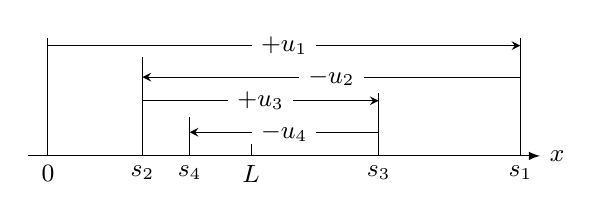
\begin{tikzpicture}[font=\small]
\pgfmathsetmacro{\k}{6}
\pgfmathsetmacro{\b}{0.2*\k}
\pgfmathsetmacro{\c}{0.7*\k}
\pgfmathsetmacro{\d}{0.3*\k}
\draw[-latex](-0.25,0)--(\k+0.25,0)node[right]{$x$};
\draw(0,0)node[below]{$0$}--++(0,1.5);
\draw(\k,0)node[below]{$s_1$}--++(0,1.5);
\draw(\b,0)node[below]{$s_2$}--++(0,1.25);
\draw(\c,0)node[below]{$s_3$}--++(0,0.8);
\draw(\d,0)node[below]{$s_4$}--++(0,0.5);
\draw(0.43*\k,0)node[below]{$L$}--++(0,0.15);
\draw[-stealth](0,1.4)--++(\k,0)node[pos=0.5,fill=white]{$+u_1$};
\draw[-stealth](\k,1)--++({\b-\k},0)node[pos=0.5,fill=white]{$-u_2$};
\draw[-stealth](\b,0.7)--++({\c-\b},0)node[pos=0.5,fill=white]{$+u_3$};
\draw[-stealth](0\c,0.3)--++({\d-\c},0)node[pos=0.5,fill=white]{$-u_4$};
\end{tikzpicture}
\caption{
اس بدلتے  تسلسل کے جزوی مجموعات جو \عددی{N=1} کے لئے مسئلہ \حوالہ{مسئلہ_تسلسل_بدلتا_تسلسل_پرکھ} کے شرائط کو مطمئن کرتا ہو۔
}
\label{شکل_تسلسل_بدلتے_ہندسی_تسلسل_کے_جزوی_مجموعات}
\end{figure}

درج ذیل کی بنا ہم مرتکز بدلتے تسلسل کے مجموعات کی قیمت  کا اندازہ  لگا سکتے ہیں۔
\begin{align*}
\abs{L-s_n}&<u_{n+1}&&n\ge N
\end{align*}

\ابتدا{مسئلہ}\شناخت{مسئلہ_تسلسل_بدلتا_اندازہ}\موٹا{بدلتے تسلسل کا مسئلہ اندازہ}\\
اگر بدلتا تسلسل \عددی{\sum_{n=1}^{\infty}(-1)^{n+1}u_n} مسئلہ \حوالہ{مسئلہ_تسلسل_بدلتا_تسلسل_پرکھ} کے تین شرائط مطمئن کرتا ہو تب \عددی{n\ge N} کے لئے  تسلسل کا مجموعہ \عددی{L} تخمیناً
\begin{align*}
s_n=u_1-u_2+\cdots+(-1)^{n+1}u_n
\end{align*}
ہو گا جس میں مطلق خلل کی قیمت \عددی{u_{n+1}} سے کم ہو گی جو پہلے غیر مستعمل جزو کی عددی قیمت ہے۔ مزید باقی \عددی{L-s_n} کی علامت وہی ہو گی جو پہلی غیر مستعمل جزو کی علامت ہو۔ 
\انتہا{مسئلہ}
%=====================

\ابتدا{مثال}
ہم مسئلہ \حوالہ{مسئلہ_تسلسل_بدلتا_اندازہ} درج ذیل تسلسل پر لاگو کرتے ہیں جس کا مجموعہ ہم جانتے ہیں۔
\begin{align*}
\sum_{n=0}^{\infty}(-1)^n\frac{1}{2^n}=1-\frac{1}{2}+\frac{1}{4}-\frac{1}{8}+\frac{1}{16}-\frac{1}{32}+\frac{1}{64}-\frac{1}{128}\,\protect\rule[-2ex]{0.1ex}{5ex}+\frac{1}{256}-\cdots
\end{align*}
یہ مسئلہ کہتا ہے کہ تسلسل کے آٹھ اجزاء لینے سے ہم  مثبت مقدار رد کرتے ہیں جس کی قیمت \عددی{\tfrac{1}{256}} سے کم ہو گی۔ ابتدائی آٹھ اجزاء کا مجموعہ \عددی{\num{0.6640625}} ہے۔ اس تسلسل کا مجموعہ درج ذیل ہے۔
\begin{align*}
\frac{1}{1-(-1/2)}=\frac{1}{3/2}=\frac{2}{3}
\end{align*}
مجموعہ اور تخمینی قیمت میں فرق \عددی{\tfrac{2}{3}-\num{0.6640625}=\num{0.0026041666}} ہے جو مثبت اور \عددی{\tfrac{1}{256}=\num{0.00390625}} سے کم ہے۔
\انتہا{مثال}
%======================

\جزوحصہء{مطلق ارتکاز}
\ابتدا{تعریف}
تسلسل \عددی{\sum a_n} اس صورت \اصطلاح{مطلق مرتکز}\فرہنگ{مرتکز!مطلق}\حاشیہب{absolutely convergent}\فرہنگ{convergent!absolute} ہو گا جب مطلق قیمتوں کا مطابقتی تسلسل \عددی{\sum \abs{a_n}} مرتکز ہو۔
\انتہا{تعریف}
%====================

ہندسی تسلسل
\begin{align*}
1-\frac{1}{2}+\frac{1}{4}-\frac{1}{8}+\cdots
\end{align*}
مطلق مرتکز ہے چونکہ مطابقتی مطلق قیمتوں کا درج ذیل تسلسل مرتکز ہے۔
\begin{align*}
1+\frac{1}{2}+\frac{1}{4}+\frac{1}{8}+\cdots
\end{align*}
بدلتا ہارمونی تسلسل مطلق مرتکز نہیں ہے چونکہ مطابقتی مطلق قیمتوں کا تسلسل (منفرج) ہارمونی تسلسل ہے۔

\ابتدا{تعریف}
جو تسلسل مرتکز ہو مگر مطلق مرتکز نہ ہو \اصطلاح{مشروط مرتکز}\فرہنگ{مرتکز!مشروط}\حاشیہب{conditional convergent}\فرہنگ{convergent!conditional} کہلاتا ہے۔
\انتہا{تعریف}
%=================

بدلتا ہارمونی تسلسل مشروط مرتکز ہے۔

مطلق ارتکاز دو وجوہات کی بنا اہم ہے۔ پہلی وجہ یہ ہے کہ ہمارے پاس مثبت اجزاء کے تسلسل کی ارتکاز کا اچھے پرکھ ہیں۔ دوسری وجہ یہ کہ کہ مطلق مرتکز تسلسل ہر صورت مرتکز ہو گا۔ یہی اگلے مسئلہ کا موضوع ہے۔

\ابتدا{مسئلہ}\شناخت{مسئلہ_تسلسل_ہر_مطلق_مرتکز_تسلسل_مرتکز}\موٹا{مطلق ارتکاز پرکھ}\\
اگر \عددی{\sum_{n=1}^{\infty}\abs{a_n}} مرتکز ہو تب \عددی{\sum_{n=1}^{\infty}a_n} مرتکز ہو گا۔
\انتہا{مسئلہ}
%=====================
\ابتدا{ثبوت}
ہر \عددی{n} کے لئے
\begin{align*}
-\abs{a_n}\le a_n\le \abs{a_n}\quad \implies \quad 0\le a_n+\abs{a_n}\le 2\abs{a_n}
\end{align*}
ہو گا۔ اگر \عددی{\sum_{n=1}^{\infty}\abs{a_n}} مرتکز ہو تب \عددی{\sum_{n=1}^{\infty}2\abs{a_n}} مرتکز ہو گا اور بلا واسطہ تقابلی پرکھ کے تحت  غیر منفی تسلسل 
\begin{align*}
\sum_{n=1}^{\infty}(a_n+\abs{a_n})
\end{align*}
بھی مرتکز ہو گا۔ ہم مساوات \عددی{a_n=(a_n+\abs{a_n})-\abs{a_n}} کی مدد سے  \عددی{\sum_{n=1}^{\infty}a_n} کو دو مرتکز تسلسل کا فرق 
\begin{align*}
\sum_{n=1}^{\infty}a_n=\sum_{n=1}^{\infty}(a_n+\abs{a_n}-\abs{a_n})=\sum_{n=1}^{\infty}(a_n+\abs{a_n})-\sum_{n=1}^{\infty}\abs{a_n}
\end{align*}
لکھ سکتے ہیں۔یوں \عددی{\sum_{n=1}^{\infty}a_n} مرتکز ہو گا۔
\انتہا{ثبوت}
%==============

ہم مسئلہ \حوالہ{مسئلہ_تسلسل_ہر_مطلق_مرتکز_تسلسل_مرتکز} کو یوں بھی پڑھ سکتے ہیں کہ ہر مطلق مرتکز تسلسل مرتکز ہو گا البتہ ضروری نہیں ہے کہ مرتکز تسلسل مطلق مرتکز ہو۔

\ابتدا{مثال}\شناخت{مثال_تسلسل_درکار_بعد_الف}
تسلسل \عددی{\sum_{n=1}^{\infty}(-1)^{n+1}\tfrac{1}{n^2}=1-\tfrac{1}{4}+\tfrac{1}{9}-\tfrac{1}{16}+\cdots} کا مطابقتی مثبت اجزاء کا تسلسل
\begin{align*}
\sum_{n=1}^{\infty}\frac{1}{n^2}=1+\frac{1}{4}+\frac{1}{9}+\frac{1}{16}+\cdots
\end{align*} 
ہے جو مرتکز ہے۔یوں اصل تسلسل اس لئے مرتکز ہے کہ یہ مطلق مرتکز ہے۔
\انتہا{مثال}
%======================
\ابتدا{مثال}
تسلسل \عددی{\sum_{n=1}^{\infty}\tfrac{\sin n}{n^2}=\tfrac{\sin 1}{1}+\tfrac{\sin 2}{4}+\tfrac{\sin 3}{9}+\cdots} کا مطابقتی مثبت اجزاء کا تسلسل درج ذیل ہے
\begin{align*}
\sum_{n=1}^{\infty}\abs{\frac{\sin n}{n^2}}=\frac{\abs{\sin 1}}{1}+\frac{\abs{\sin 2}}{4}+\frac{\abs{\sin 3}}{9}+\cdots
\end{align*}
جس کا ارتکاز  \عددی{\sum_{n=1}^{\infty}\tfrac{1}{n^2}} کے ساتھ موازنہ کرنے سے دیکھا جا سکتا ہے جہاں ہر \عددی{n} کے لئے \عددی{\abs{\sin n}\le 1} ہو گا۔ چونکہ اصل تسلسل مطلق مرتکز ہے، لہٰذا یہ مرتکز ہو گا۔
\انتہا{مثال}
%======================
\ابتدا{مثال}\موٹا{بدلتا \عددی{p} تسلسل}\\
مثبت مستقل \عددی{p} کی صورت میں ترتیب \عددی{\{\tfrac{1}{n^p}\}}  گھٹتا ترتیب ہے جس کا حد صفر ہے۔ یوں بدلتا \عددی{p} تسلسل
\begin{align*}
\sum_{n=1}^{\infty}\frac{(-1)^{n-1}}{n^p}=1-\frac{1}{2^p}+\frac{1}{3^p}-\frac{1}{4^p}+\cdots,\quad p>0
\end{align*}
مرتکز ہو گا۔

اگر \عددی{p>1} ہو تب یہ مطلق مرتکز تسلسل ہو گا۔ اگر \عددی{p\le 1} ہو تب یہ مشروط مرتکز تسلسل ہو گا۔
\begin{align*}
1-\frac{1}{\sqrt{2}}+\frac{1}{\sqrt{3}}-\frac{1}{\sqrt{4}}+\cdots&&\text{\RL{مشروط مرتکز}}\\
1-\frac{1}{2^{3/2}}+\frac{1}{3^{3/2}}-\frac{1}{4^{3/2}}+\cdots&&\text{\RL{مطلق مرتکز}}
\end{align*}
\انتہا{مثال}
%===================

\جزوحصہء{تسلسل کی ترتیب نو}
\ابتدا{مسئلہ}\موٹا{مطلق مرتکز تسلسل کا مسئلہ ترتیب نو}\\
اگر \عددی{\sum_{n=1}^{\infty}a_n} مطلق مرتکز ہو اور ترتیب \عددی{\{a_n\}} کے اجزاء کی ترتیب نو  کر کے انہیں \عددی{b_1,b_2,\cdots,b_n,\cdots}  لکھا جائے تب \عددی{\sum b_n} مطلق مرتکز ہو گا اور درج ذیل ہو گا۔
\begin{align*}
\sum_{n=1}^{\infty}a_n=\sum_{n=1}^{\infty}b_n
\end{align*}
\انتہا{مسئلہ}
%==================

\ابتدا{مثال}
ہم نے مثال \حوالہ{مثال_تسلسل_درکار_بعد_الف} میں دیکھا کہ تسلسل
\begin{align*}
1-\frac{1}{4}+\frac{1}{9}-\frac{1}{16}+\cdots+(-1)^{n-1}\frac{1}{n^2}+\cdots
\end{align*}
مطلق مرتکز ہے۔ اس کی ترتیب نو کرتے ہوئے ابتدائی جزو مثبت اور اس  کے بعد دو منفی اجزاء منتخب کیے جا سکتے ہیں۔اس کے بعد تین مثبت اور چار منفی اجزاء  منتخب کیے جا سکتے ہیں، وغیرہ وغیرہ۔ یوں ایک ہی علامت کے \عددی{k} اجزاء کے بعد الٹ علامت کے \عددی{k+1} اجزاء ہوں گے۔ ایسے تسلسل کے ابتدائی دس اجزاء درج ذیل ہوں گے۔
\begin{align*}
1-\frac{1}{4}-\frac{1}{16}+\frac{1}{9}+\frac{1}{25}+\frac{1}{49}-\frac{1}{36}-\frac{1}{64}-\frac{1}{100}-\frac{1}{144}+\cdots
\end{align*}
مسئلہ ترتیب نو کے تحت دونوں تسلسل ایک ہی عدد پر مرتکز ہوں گے۔ اس مثال میں (اگر ہم جانتے کہ ایسا ممکن ہے) ہم خوشی سے دوسرے تسلسل کی جگہ پہلا تسلسل استعمال کرنا چاہیں گے۔ اس سے بھی بہتر ہوتا اگر ہم جانتے کہ ان دونوں تسلسل کا مجموعہ درج ذیل کے برابر ہے۔
\begin{align*}
\sum_{n=1}^{\infty}\frac{1}{(2n-1)^2}-\sum_{n=1}^{\infty}\frac{1}{(2n)^2}
\end{align*}
\انتہا{مثال}
%======================
